\problemname{Triangle numbers}
\noindent
In a class with $N$ students, it is time for the obligatory task of giving a speech.
Most students are very excited to give their speeches and can hardly wait for their turn.
First, they must be divided into three groups. Everyone in group $1$ will then present to group $2$,
group $2$ to group $3$, and group $3$ to group $1$.

One complication in this grouping is that the students have different ambition levels. Each student $i$
requires to give their speech to at least $A_i$ people.
So, if student $i$ ends up in group $1$, group $2$ must have at least $A_i$ members for student $i$ to be satisfied.

\begin{figure}[!h]
  \centering
  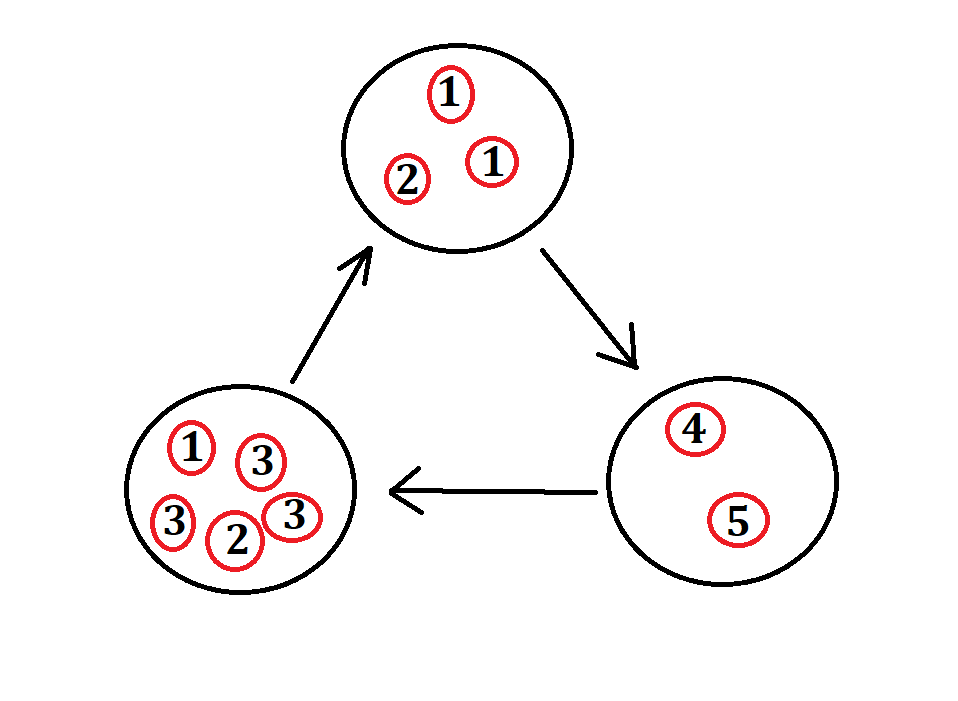
\includegraphics[width=6cm]{triangeltal.png}
  \caption{The image corresponds to the first example.}
\end{figure}

Your task is to determine, given the students' ambition levels, if there is a way to divide the students into three groups so that everyone is satisfied, and if so, find a valid division.

\section*{Input}
The first line contains an integer $N$ ($3 \leq N \leq 5 \cdot 10^5$), the number of students in the class.

The second line contains $N$ integers $A_i$ ($1 \leq A_i \leq N$), where $A_i$ is the minimum number of students the $i$-th student wants to give a speech to.

\section*{Output}
If there is no valid division, print a single line with the string ``\texttt{NO}''.

If there is a valid division, first print a line with the string ``\texttt{YES}''.
Then, print a line with a string $S$ consisting of the characters \texttt{1}, \texttt{2}, and \texttt{3}.
The character at position $i$ in this string indicates which group student $i$ belongs to. If there are multiple solutions, you can print any of them.

\section*{Points}
Your solution will be tested on several test case groups.
To get the points for a group, it must pass all the test cases in the group.

\noindent
\begin{tabular}{| l | l | l |}
  \hline
  \textbf{Group} & \textbf{Point value} & \textbf{Constraints} \\ \hline
  $1$   & $14$       & $A_1 = A_2 = \cdots = A_N$\\ \hline
  $2$   & $16$       & $N \leq 10$  \\ \hline
  $3$   & $11$       & $A_i \leq 3$ \\ \hline
  $4$   & $23$       & $N \leq 3000$ \\ \hline
  $5$   & $36$       & No additional constraints. \\ \hline
\end{tabular}


